%%%%%%%%%%%%%%%%%%%%%%%%%%%%%%%%%%%%%%%%%
% Jacobs Landscape Poster
% LaTeX Template
% Version 1.1 (14/06/14)
%
% Created by:
% Computational Physics and Biophysics Group, Jacobs University
% https://teamwork.jacobs-university.de:8443/confluence/display/CoPandBiG/LaTeX+Poster
% 
% Further modified by:
% Nathaniel Johnston (nathaniel@njohnston.ca)
%
% This template has been downloaded from:
% http://www.LaTeXTemplates.com
%
% License:
% CC BY-NC-SA 3.0 (http://creativecommons.org/licenses/by-nc-sa/3.0/)
%
%%%%%%%%%%%%%%%%%%%%%%%%%%%%%%%%%%%%%%%%%

%----------------------------------------------------------------------------------------
%	PACKAGES AND OTHER DOCUMENT CONFIGURATIONS
%----------------------------------------------------------------------------------------

\documentclass[final]{beamer}

\usepackage{amsmath}
\usepackage{graphicx}
\usepackage{blindtext}
\usepackage[scale=1.24]{beamerposter} % Use the beamerposter package for laying out the poster

\usetheme{confposter} % Use the confposter theme supplied with this template

\setbeamercolor{block title}{fg=ngreen,bg=white} % Colors of the block titles
\setbeamercolor{block body}{fg=black,bg=white} % Colors of the body of blocks
\setbeamercolor{block alerted title}{fg=white,bg=dblue!70} % Colors of the highlighted block titles
\setbeamercolor{block alerted body}{fg=black,bg=dblue!10} % Colors of the body of highlighted blocks
% Many more colors are available for use in beamerthemeconfposter.sty

%-----------------------------------------------------------
% Define the column widths and overall poster size
% To set effective sepwid, onecolwid and twocolwid values, first choose how many columns you want and how much separation you want between columns
% In this template, the separation width chosen is 0.024 of the paper width and a 4-column layout
% onecolwid should therefore be (1-(# of columns+1)*sepwid)/# of columns e.g. (1-(4+1)*0.024)/4 = 0.22
% Set twocolwid to be (2*onecolwid)+sepwid = 0.464
% Set threecolwid to be (3*onecolwid)+2*sepwid = 0.708

\newlength{\sepwid}
\newlength{\onecolwid}
\newlength{\twocolwid}
\newlength{\threecolwid}
\setlength{\paperwidth}{48in} % A0 width: 46.8in
\setlength{\paperheight}{36in} % A0 height: 33.1in
\setlength{\sepwid}{0.024\paperwidth} % Separation width (white space) between columns
\setlength{\onecolwid}{0.22\paperwidth} % Width of one column
\setlength{\twocolwid}{0.464\paperwidth} % Width of two columns
\setlength{\threecolwid}{0.708\paperwidth} % Width of three columns
\setlength{\topmargin}{-0.5in} % Reduce the top margin size
%-----------------------------------------------------------

\usepackage{graphicx}  % Required for including images

\usepackage{booktabs} % Top and bottom rules for tables

%----------------------------------------------------------------------------------------
%	TITLE SECTION 
%----------------------------------------------------------------------------------------

\title{Multivariate Skew-Normal Mixture Model for Infant Development Clustering} % Poster title

\author{Carter Allen$^1$; Brian Neelon, PhD$^1$; Sara E. Benjamin-Neelon, PhD, JD, MPH$^2$} % Author(s)

\institute{$^1$Department of Public Health Sciences, Medical University of South Carolina; $^2$Bloomberg School of Public Health, Johns Hopkins University}

%----------------------------------------------------------------------------------------

\begin{document}

\addtobeamertemplate{block end}{}{\vspace*{2ex}} % White space under blocks
\addtobeamertemplate{block alerted end}{}{\vspace*{2ex}} % White space under highlighted (alert) blocks

\setlength{\belowcaptionskip}{2ex} % White space under figures
\setlength\belowdisplayshortskip{2ex} % White space under equations

\begin{frame}[t] % The whole poster is enclosed in one beamer frame

\begin{columns}[t] % The whole poster consists of three major columns, the second of which is split into two columns twice - the [t] option aligns each column's content to the top

\begin{column}{\sepwid}\end{column} % Empty spacer column

\begin{column}{\onecolwid} % The first column

%----------------------------------------------------------------------------------------
%	OBJECTIVES
%----------------------------------------------------------------------------------------

\begin{alertblock}{Abstract}
 
We propose a novel Bayesian model for infant development patterns that addresses primary research questions in this area while allowing for skewness and correlation of outcomes. Our model is based on finite mixtures of multivariate skew normal (MSN) distributions, where covariates are allowed on both the multivariate outcomes and probability of latent class membership. We also allow for missing outcome data by imputing missing outcomes from their conditional multivariate normal distributions. We demonstrate our method using data from the Nurture study.

\end{alertblock}

%----------------------------------------------------------------------------------------
%	INTRODUCTION
%----------------------------------------------------------------------------------------

\begin{block}{Introduction}

A primary goal in infant development research is to identify \textbf{latent development classes} and explain class membership in relation to covariates of interest. It is often also of interest to relate covariates to mean longitudinal growth patterns. Infant development data are inherently correlated longitudinally, often skewed, and frequently missing due to longitudinal attrition and standard practices are ill-suited for such analyses because they fail to account for one or more of these features of the data. 

\end{block}

%------------------------------------------------

\begin{block}{Motivation}
\begin{figure}
\includegraphics[width=0.9\linewidth]{bayley_dens.jpg}
\caption{Residuals of repeated measures model of Bayley motor development scores for infants at 3, 6, 9 and 12 months of age.}
\end{figure}
\end{block}

%----------------------------------------------------------------------------------------

\end{column} % End of the first column

\begin{column}{\sepwid}\end{column} % Empty spacer column

\begin{column}{\twocolwid} % Begin a column which is two columns wide (column 2)

\begin{columns}[t,totalwidth=\twocolwid] % Split up the two columns wide column

\begin{column}{\onecolwid}\vspace{-.6in} % The first column within column 2 (column 2.1)

%----------------------------------------------------------------------------------------
%	
%----------------------------------------------------------------------------------------

\begin{block}{Clustering}

A primary concern of our model is with identification of latent infant development clusters. We accomplish this via multinomial logit regression model on cluster membership, which utilizes P\'{o}lya-Gamma data-aumentation to allow for updating of all parameters using Gibbs sampling. The multinomial logit model is as follows for $l = 1,...,h$.

$$P(Z_i = l|w_i) = \pi_{il} = \frac{e^{w_i^T \delta_l}}{\sum_{r = 1}^h e^{w_i^T \delta_r}}$$

where $Z_i$ is a latent clustering indicator, $w_i$ is the vector of class probability covariates for subject $i$ ($i = 1,...,n$), $\delta_l$ contains the multinomial regression parameters for class $l$, and $h$ is the number of putative clusters specified \textit{a priori}. During MCMC estimation, class labels $Z_i$ are updated from used as class assignments in the remaining MCMC steps.

\end{block}

%----------------------------------------------------------------------------------------

\end{column} % End of column 2.1

\begin{column}{\onecolwid}\vspace{-.6in} % The second column within column 2 (column 2.2)

%----------------------------------------------------------------------------------------
%	METHODS
%----------------------------------------------------------------------------------------

\begin{block}{Conditional Imputation}

We allow for missingness of outcomes in the MSN mixture model by imputing missing values from their conditional multivariate normal distributions. We note that

$$Y_i|X_i,t_i,\boldsymbol\beta,\psi \sim N_k(X_i \boldsymbol\beta + t_i \psi, \boldsymbol\Sigma)$$

This allows us to appeal to standard conditional forms of the multivariate normal distribution. Let $Y_i = [Y^{miss}_{i_{q \times 1}} | Y^{obs}_{i_{k - q \times 1}}]^T$. We have

$$Y_i^{miss}|Y_i^{obs},X_i,t_i,\boldsymbol\beta,\psi \sim N(\mu^{miss},\boldsymbol\Sigma^{miss})$$

where $\mu^{miss}$ and $\Sigma^{miss}$ take standard forms. Each missing outcome is imputed "online", i.e. once per MCMC iteration. This provides more opportunities to explore the parameter space than multiple imputation and avoids multiplicative run-time scaling in $m$, the number of imputations.

\end{block}

%----------------------------------------------------------------------------------------

\end{column} % End of column 2.2

\end{columns} % End of the split of column 2 - any content after this will now take up 2 columns width

%----------------------------------------------------------------------------------------
%	IMPORTANT RESULT
%----------------------------------------------------------------------------------------

\begin{alertblock}{Important Results}

We developed a novel Bayesian MSN mixture model, and showed superior performance compared to standard approaches. We applied the MSN mixture model to data from the Nurture study and discovered three distinct development classes characterized by differences in development trajectories and demographics.

\end{alertblock} 

%----------------------------------------------------------------------------------------

\begin{columns}[t,totalwidth=\twocolwid] % Split up the two columns wide column again

\begin{column}{\onecolwid} % The first column within column 2 (column 2.1)

%----------------------------------------------------------------------------------------
%	MATHEMATICAL SECTION
%----------------------------------------------------------------------------------------

\begin{block}{MSN Regression}

We model the effect of covariates on longitudinal development outcomes through the use of a MSN regression model. The MSN distribution can be represented as a multivariate normal random variable with a latent truncated normal random effect, $t$. Let $\mathbf{y}_{i}$ be the $k \times 1$ outcome vector for subject $i$.

$$\mathbf{y}_{i} = \boldsymbol\beta^T \mathbf{x}_{i} + t_{i}\boldsymbol\psi + \boldsymbol\epsilon_{i}$$

where $\mathbf{x}_i$ is the $p \times 1$ vector of covariate values for subject $i$, $\boldsymbol\beta$ is the $p \times k$ vector of fixed effects coefficients , $t_i \stackrel{iid}{\sim} N_{[0,\infty)}(0,1)$ is a conditional truncated normal random effect, $\psi_l$ is the vector containing cluster-specific skewness parameters for each timepoint, and $\boldsymbol\epsilon_i \sim N_k(0,\boldsymbol\Sigma_{k \times k})$ is the correlated error term.

\end{block}

%----------------------------------------------------------------------------------------

\end{column} % End of column 2.1

\begin{column}{\onecolwid} % The second column within column 2 (column 2.2)

%----------------------------------------------------------------------------------------
%	RESULTS
%----------------------------------------------------------------------------------------

\begin{block}{Simulation Study}

\begin{table}[t]

\caption{\label{tab:unnamed-chunk-4}Parameter estimates for n = 1000, k = 4, p = 2, h = 3, v = 3 simulation.}
\centering
\fontsize{20}{20}\selectfont
\begin{tabular}{llllllll}
\toprule
\multicolumn{2}{c}{ } & \multicolumn{2}{c}{Class 1} & \multicolumn{2}{c}{Class 2} & \multicolumn{2}{c}{Class 3} \\
\cmidrule(l{3pt}r{3pt}){3-4} \cmidrule(l{3pt}r{3pt}){5-6} \cmidrule(l{3pt}r{3pt}){7-8}
Component & Parm. & True & Est. (95\% CrI) & True & Est. (95\% CrI) & True & Est. (95\% CrI)\\
\midrule
\addlinespace[0.3em]
\multicolumn{8}{l}{\textbf{ }}\\
\hspace{1em}MSN & $\beta_{11}$ & -0.54 & -0.51 (-0.61, -0.41) & -0.19 & -0.22 (-0.35, -0.09) & 1.84 & 1.81 (1.65, 1.99)\\
\hspace{1em}Reg. & $\beta_{12}$ & -1.06 & -1.07 (-1.15, -0.98) & -0.16 & -0.13 (-0.25, -0.02) & 2.03 & 2.09 (1.93, 2.23)\\
\hspace{1em} & $\beta_{13}$ & -1.28 & -1.22 (-1.32, -1.11) & 0.59 & 0.58 (0.46, 0.69) & 1.8 & 1.74 (1.58, 1.9)\\
\hspace{1em} & $\beta_{14}$ & -1.91 & -1.83 (-1.92, -1.74) & -0.2 & -0.12 (-0.25, -0.01) & 1.43 & 1.37 (1.22, 1.52)\\

\addlinespace[0.3em]
\multicolumn{8}{l}{\textbf{ }}\\
\hspace{1em} & $\sigma^2_{11}$ & 1 & 0.9 (0.78, 1.03) & 1 & 1.04 (0.88, 1.26) & 1 & 1.39 (1.08, 1.76)\\
\hspace{1em} & $\sigma^2_{12}$ & -0.1 & -0.12 (-0.22, -0.02) & -0.32 & -0.31 (-0.44, -0.18) & 0.08 & 0.27 (0.04, 0.52)\\
\hspace{1em} & $\sigma^2_{13}$ & -0.18 & -0.17 (-0.28, -0.08) & -0.52 & -0.5 (-0.66, -0.38) & 0.78 & 1.19 (0.87, 1.54)\\
\hspace{1em} & $\sigma^2_{14}$ & 0.39 & 0.31 (0.22, 0.43) & 0.04 & 0.05 (-0.07, 0.22) & 0.41 & 0.72 (0.47, 0.99)\\
\hspace{1em} & $\sigma^2_{22}$ & 1 & 0.97 (0.84, 1.12) & 1 & 0.94 (0.77, 1.14) & 1 & 1.18 (0.91, 1.5)\\

\addlinespace[0.3em]
\multicolumn{8}{l}{\textbf{ }}\\
\hspace{1em} & $\psi_{1}$ & -0.33 & -0.28 (-0.4, -0.18) & 0.67 & 0.64 (0.5, 0.78) & -1 & -0.91 (-1.12, -0.68)\\
\hspace{1em} & $\psi_{2}$ & -0.33 & -0.21 (-0.34, -0.09) & 0.67 & 0.7 (0.55, 0.84) & -1 & -0.96 (-1.16, -0.76)\\
\hspace{1em} & $\psi_{3}$ & -0.33 & -0.27 (-0.39, -0.14) & 0.67 & 0.72 (0.58, 0.86) & -1 & -0.91 (-1.14, -0.69)\\
\hspace{1em} & $\psi_{4}$ & -0.33 & -0.18 (-0.3, -0.07) & 0.67 & 0.73 (0.6, 0.87) & -1 & -0.93 (-1.13, -0.73)\\
\addlinespace[0.3em]
\multicolumn{8}{l}{\textbf{ }}\\
\hspace{1em}Multi. & $\delta_{11}$ & -0.53 & -0.5 (-0.74, -0.24) & -0.53 & -0.5 (-0.74, -0.24) & -0.53 & -0.5 (-0.74, -0.24)\\
\hspace{1em}Logit & $\delta_{12}$ & 0.44 & 0.28 (0.02, 0.56) & 0.44 & 0.28 (0.02, 0.56) & 0.44 & 0.28 (0.02, 0.56)\\
\hspace{1em} & $\delta_{21}$ & 0.34 & 0.38 (0.09, 0.63) & 0.34 & 0.38 (0.09, 0.63) & 0.34 & 0.38 (0.09, 0.63)\\
\addlinespace[0.3em]
\multicolumn{8}{l}{\textbf{ }}\\
\hspace{1em}Clust. & $\pi_l$ & 0.41 & 0.41 (0.4, 0.42) & 0.36 & 0.36 (0.35, 0.37) & 0.23 & 0.23 (0.22, 0.24)\\
\bottomrule
\end{tabular}
\end{table}

\end{block}

%----------------------------------------------------------------------------------------

\end{column} % End of column 2.2

\end{columns} % End of the split of column 2

\end{column} % End of the second column

\begin{column}{\sepwid}\end{column} % Empty spacer column

\begin{column}{\onecolwid} % The third column

%----------------------------------------------------------------------------------------
%	CONCLUSION
%----------------------------------------------------------------------------------------

\begin{block}{Application Results}

\begin{table}[]
\caption{\label{tab:unnamed-chunk-4}Estimated effects of sex and race on odds of cluster membership relative to the reference cluster.}
\centering
\fontsize{30}{30}\selectfont
\def\arraystretch{1.5}
\begin{tabular}{llll}
\hline
Variable & \multicolumn{1}{c}{\begin{tabular}[c]{@{}c@{}}Class 1\\ $\hat{\text{OR}}$ (95\% CrI)\end{tabular}} & \multicolumn{1}{c}{\begin{tabular}[c]{@{}c@{}}Class 2\\ $\hat{\text{OR}}$ (95\% CrI)\end{tabular}} & \multicolumn{1}{c}{\begin{tabular}[c]{@{}c@{}}Class 3\\ $\hat{\text{OR}}$ (95\% CrI)\end{tabular}} \\ \hline
Sex (F) & 1.80 (1.20, 3.16) & 1.25 (0.96, 1.81) & 1.42 (1.10, 2.03) \\
Race (W) & 1.57 (1.07, 2.80) & 1.44 (1.07, 2.13) & 1.41 (1.04, 2.04) \\ \hline
\end{tabular}
\end{table}

\

In Table 2, we demonstrate the capability of estimating the effect of covariates (race and sex here) on posterior odds of cluster membership. 

\begin{figure}
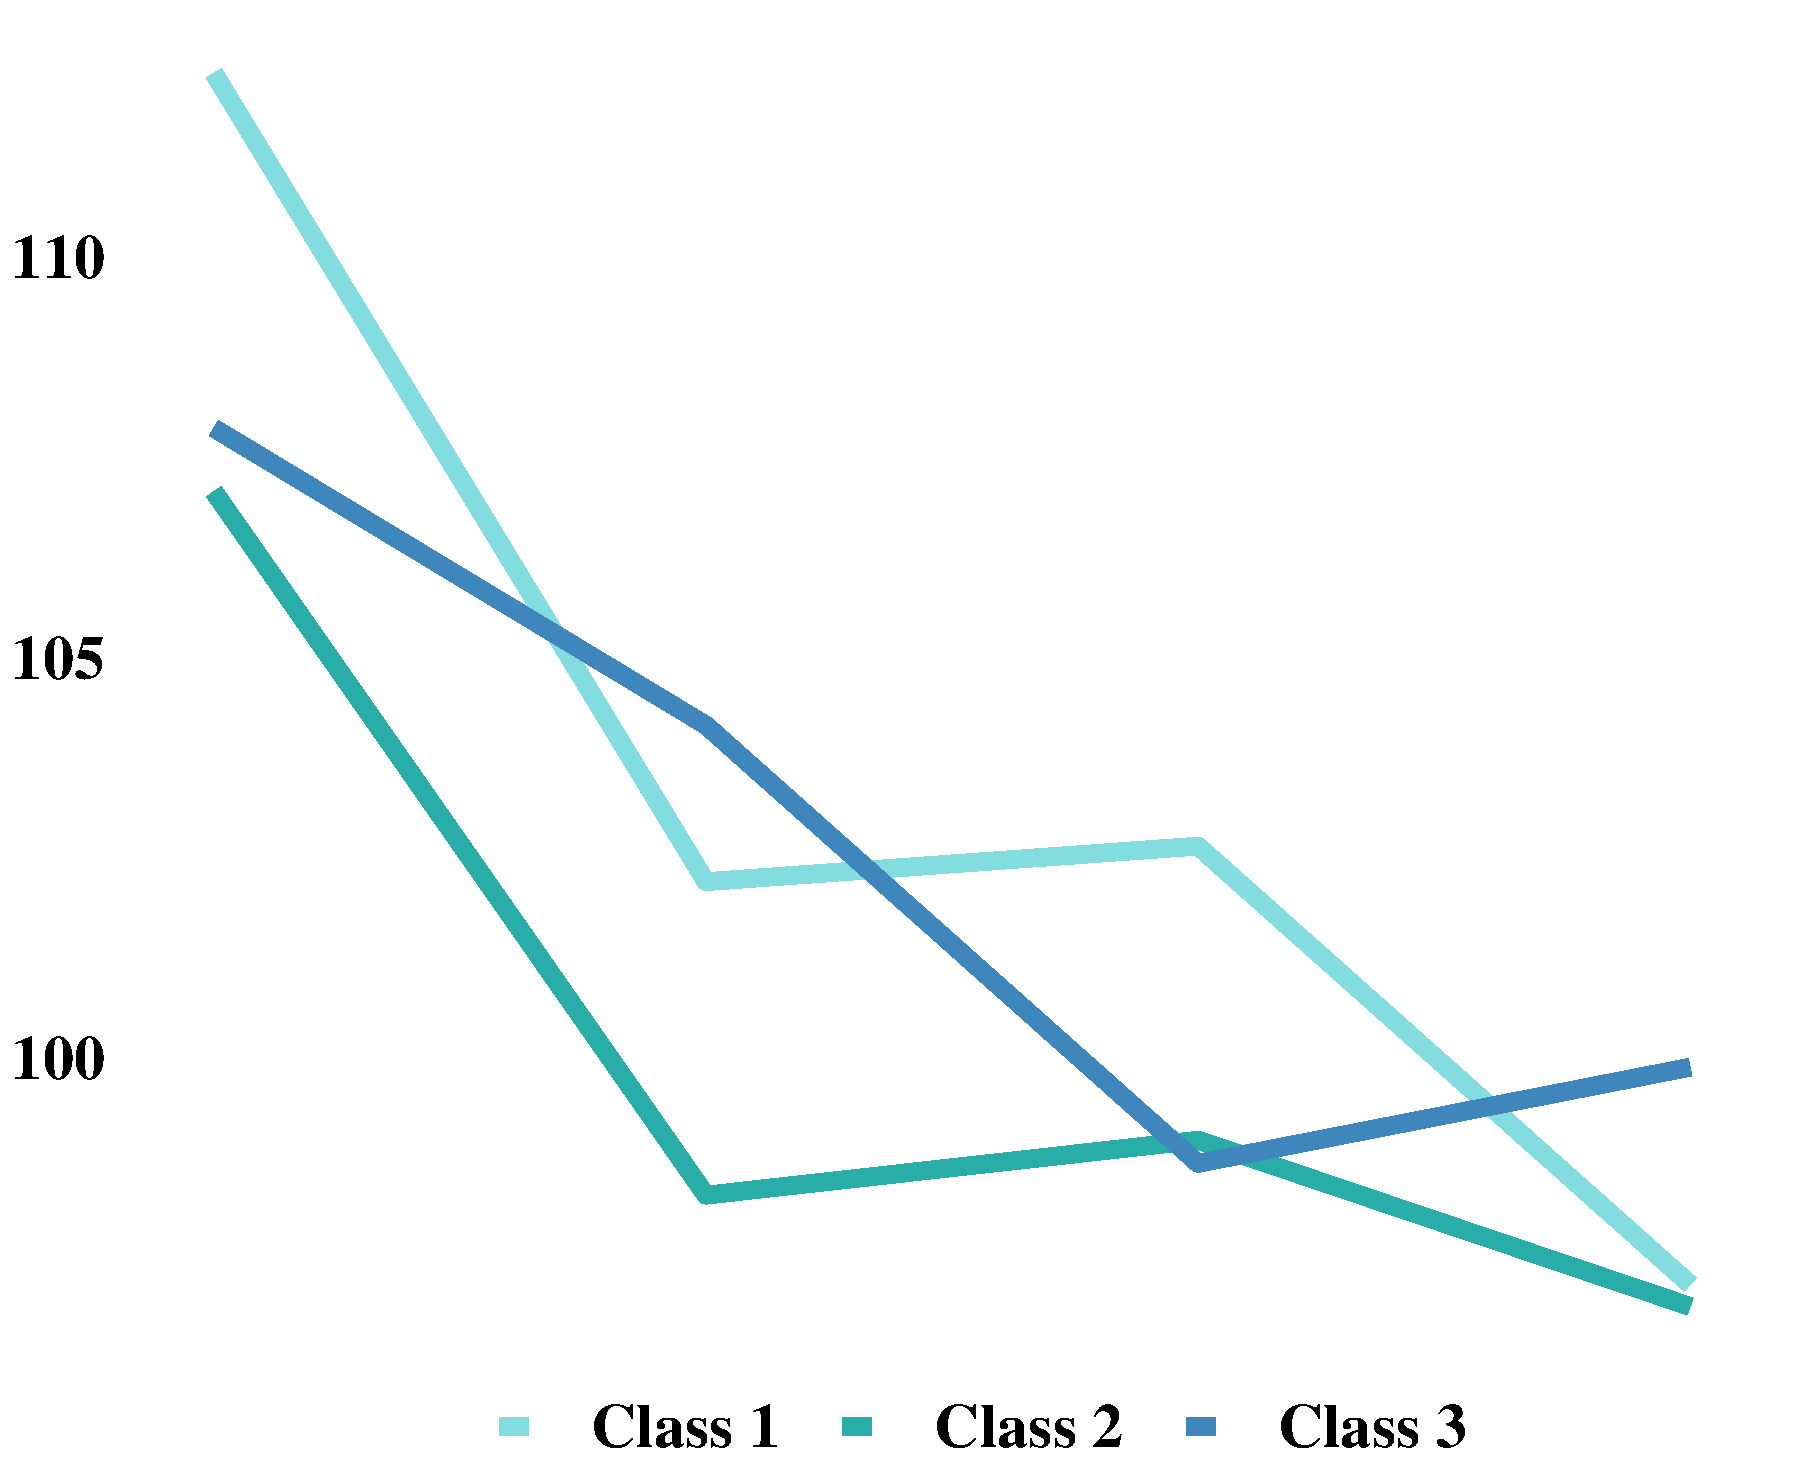
\includegraphics[height=0.8\linewidth,width=1\linewidth]{clust_trends.pdf}
\caption{Mean development patterns in each estimated class}
\end{figure}

Above is a plot of the mean Bayley score for each of the fitted clusters. We observe similar development patterns but different baseline development between clusters 1 and 2, and a qualitatively different development pattern in cluster 3 than in the clusters 1 and 2. 


\end{block}



%----------------------------------------------------------------------------------------
%	REFERENCES
%----------------------------------------------------------------------------------------


%----------------------------------------------------------------------------------------
%	ACKNOWLEDGEMENTS
%----------------------------------------------------------------------------------------


%----------------------------------------------------------------------------------------
%	CONTACT INFORMATION
%----------------------------------------------------------------------------------------

\setbeamercolor{block alerted title}{fg=black,bg=norange} % Change the alert block title colors
\setbeamercolor{block alerted body}{fg=black,bg=white} % Change the alert block body colors




\begin{alertblock}{Further Resources}

\centering
https://carter-allen.github.io/MVSN-FMM

\end{alertblock}

\tiny  \textbf{(1) Fruhwirth-Schnatter, S and Pyne, S. (2010)}. Bayesian inference for finite mixtures of univariate and multivariate skew-normal and skew-t distributions. Biostatistics. 2010 Jan 27;11(2):317- 36.

\textbf{(2) Benjamin-Neelon SE, Ostbye T, Bennett GG, et al.} Cohort profile for the Nurture Observational Study examining associations of multiple caregivers on infant growth in the Southeastern USA. BMJ open. 2017 Feb 1;7(2):e013939.

\

\tiny \textbf{Funding:} \textit{This work is supported by a grant from the NIH (\textbf{R01DK094841}) and a grand from the NLM (\textbf{1R21LM012866-01})}.




%----------------------------------------------------------------------------------------

\end{column} % End of the third column

\end{columns} % End of all the columns in the poster

\end{frame} % End of the enclosing frame

\end{document}
